\documentclass[conference]{IEEEtran}
\IEEEoverridecommandlockouts
% The preceding line is only needed to identify funding in the first footnote. If that is unneeded, please comment it out.
\usepackage{cite}
\usepackage{amsmath,amssymb,amsfonts}
\usepackage{algorithmic}
\usepackage{graphicx}
\usepackage{textcomp}
\usepackage{xcolor}
\def\BibTeX{{\rm B\kern-.05em{\sc i\kern-.025em b}\kern-.08em
    T\kern-.1667em\lower.7ex\hbox{E}\kern-.125emX}}
\begin{document}

\title{Recycling Assistant\\
{\footnotesize \textsuperscript{}Identifying and Categorizing Objects based on Recyclability}
}

\author{\IEEEauthorblockN{Doo Woong Chung}
\IEEEauthorblockA{\textit{Dept. Information Systems} \\
\textit{Hanyang University}\\
Seoul, South Korea \\
dwchung@hanyang.ac.kr}
\and
\IEEEauthorblockN{Kim Soohyun}
\IEEEauthorblockA{\textit{Dept. Information Systems} \\
\textit{Hanyang University}\\
Seoul, South Korea \\
soowithwoo@gmail.com}
\and
\IEEEauthorblockN{Lim Hongrok}
\IEEEauthorblockA{\textit{Dept. Information Systems} \\
\textit{Hanyang University}\\
Seoul, South Korea \\
hongrr123@gmail.com}
}

\maketitle

\begin{abstract}
Sometimes being able to correctly identify and understand how to recycle certain items can be difficult. As such, the Recycling Assistant hopes to be able to alleviate some of those questions, via the identification and categorization of more common objects.

An observation that can be made is that certain recyclable items are not often disposed of an in efficient manner - such as plastic bottles not being emptied of air - causing a lot of empty volume. As a result, an additional feature that the Recycling Assistant hopes to implement is notifying the user when an item can be disposed of in a more optimal manner.
\end{abstract}

\begin{IEEEkeywords}
identification, detection, classification, opencv, recycling, waste
\end{IEEEkeywords}

\section{Role Assignments}
Below is the table of external role assignments for this project. Due to the small team size, the development manager position has been split between the software developers, in order to facilitate quick decision making.
\newline

\begin{table}[htbp!]\normalsize
\begin{center}
\begin{tabular}{|p{1.5cm}|p{1.7cm}|p{4.5cm}|}
\hline
\textbf{Name} & \textbf{\textit{Role}}& \textbf{\textit{Responsibilities}}\\
\hline
Doo Woong Chung & Co-Development Manager \& Software Developer &
Responsible for assigning tasks and identifying the next step in the project/what needs to be done to stay on track, and converting requirements into tangible functionality. In addition, they are also responsible for identifying frameworks that would work best with the project.\newline
\newline Responsible for implementing software functionality and collaborating with other Software Developers in order to fulfill and push required features. Also responsible for maintaining code and coordinating pull requests.
\\ \hline
\end{tabular}
\label{tab1}
\end{center}
\end{table}
\newpage

\begin{table}[htbp!]\normalsize
\begin{center}
\begin{tabular}{|p{1.5cm}|p{1.7cm}|p{4.5cm}|}
\hline
\textbf{Name} & \textbf{\textit{Role}}& \textbf{\textit{Responsibilities}}\\
\hline
Kim Soohyun & User \& Customer &
Responsible for testing the application, and pointing out any flaws in the application that may requirement improvement.\newline
\newline In addition, they are responsible for providing feedback in how to improve upon those flaws in order, as well as continuously checking off on whether the requirements are being fulfilled. 
\newline In the event that the requirements do not seem to be fulfilled at a reasonable level, they are responsible for relaying actionable feedback, and evaluating implemented features.
\\ \hline
Lim Hongrok & Co-Development Manager \& Software Developer &
Responsible for implementing software functionality and collaborating with other Software Developers in order to fulfill and push required features.\newline
\newline In addition, they are responsible for keeping things grounded, and making sure that the minimum viable product is on track. 
\newline They are also responsible for communicating with the user and customer to receive and incorporate feedback into the product. Also responsible for maintaining code and coordinating pull requests.
\\ \hline
\end{tabular}
\label{tab1}
\end{center}
\end{table}

\newpage

\section{Introduction}
\subsection{Problem Statement}
The Recycling Assistant is a project hoping to identify, and categorize recyclable materials. In this form, we envision the Recycling Assistant to allow the user to hold up an item and display which category of recycling the item belongs in. In the event that the item is not recyclable, it will notify the user accordingly. In addition, if there is an additional tip for that category (ie. detected bottle) it will notify the user that an optimal method of recycling the item would be to minimize its volume (crushing it). \\
Recycling can be a convoluted topic at times, with people sometimes confusing what is recyclable and what is not. As a result, objects are often incorrectly disposed of, with either recyclables ending up in general waste, or objects that aren't recyclable, heading to the recycling plant. For example, hybrid materials is often the case, or confusion regarding the actual material of the object. This leads to only a fraction of the submitted recycled waste actually being able to be recycled, with the remainder heading back to landfills. \\

Our goal is to provide an assistant program that can quickly guide the user to which type of category of recycling the item that the user shows the camera, belongs in - if it is recyclable to begin with. Otherwise, they will be notified that it is more fitted to general waste, or unknown. This would help cut down on the issue of the user either not being sure of whether the object is recyclable and disposing of it in general waste, as well as help provide the user with helpful tips on how to optimize their recycle behavior.\\
We hope to also be able to incorporate the detection of different materials in a way such that the Assistant can differentiate between several types of material on the same object, and inform the user on why the object would not be recyclable in its current state (ie. Plastic film on a paper box is detected).\\

\subsection{Client's problem}
In the case of apartment, communal living facilities, and companies that live in common, recycling is somtimes difficult due to lack of responsibility from people. In this case, the recycling assistant may operate as a system that recommends proper recyling. \\

Recycling assistant can also have a positive effect on childrend's recycling education. Recycling with parents using recycling assistant can educate children about environment and teach them the right way to recycle. As a result, recycling assistants can be a teaching tool that promotes people's environmental awareness and helps children's environmental education by being introduced in schools.

\subsection{Motivation}

The idea for this project stems from the observation that recycling, while seemingly a simple topic from an external point of view, can get confusing with certain types of objects. For example, as a mixture of different materials are often used in products these days, it is sometimes confusing to tell if an object is really recyclable or not. \\
In addition, as AI/ML usage in environmentally friendly initiatives is a topic of high interest, waste-related datasets are plentiful, and we hope to leverage these datasets in order to train something that would help users with a quick and easy way to optimize their recycling behavior, while also providing useful statistics.\\

While there are a fair amount of similar, existing projects, they are targeted towards commercial/industrial applications, and are typically not open source. Thus, we were motivated to provide an open-source alternative application for users to be able to run themselves.\\

Our application focuses on providing people with the convenience of being able to quickly consult with the application and receive feedback on how an object is classified in terms of recyclability, in addition to receiving any potential tips to with regards to their disposal patterns. \\
As a result, we hope that this application will help reduce the problem of incorrectly recycled objects occurring, or recyclable objects being sent to the landfill from a normal consumer user standpoint. \\~\\

\section{Existing Products}

There are quite a bit of related existing products for this Recycling related AI work, as it is a field of interest in both the AI sector, as well as having a positive environmental affect. However, they generally range from proprietary solutions, or projects that are not open source.

In general, they seem to generally be integrated into specialized commercial applications, or proof of concepts.
\newline

\subsection{Recycle Mate \textsuperscript{[1]}}

An Android/iOS application which scans an item, and identifies which bin it goes into. It is highly localized, directing users into the correct bin to dispose of based on information provided by the local council - thus, it is limited to residents in New South Wales only. It takes a picture of the item, analyzes it and directs the user to which color bin it needs to be disposed of in.

Recycle Mate is not open source, and often receives feedback that the picture system is clunky, as well as unhelpful to residents residing outside of New South Wales.
\newline

\subsection{Bin-e Smart Waste Bin \textsuperscript{[2]}}

A "Smart Recycling Bin", which automatically sorts the inserted item into the correct bin. It uses an inserted camera alongside object recognition in order to correctly sort the item. It is described as an "IOT device which sorts and compresses the recyclables automatically, combining unique AI-based object recognition..."

In a sense, Bin-e's system works similarly to what we are looking to achieve, aside from the IOT device integration.
\newline

\subsection{World Waste Platform \textsuperscript{[3]}}

The "Let's Do It AI Project" is a project developed in conjunction with the Let's Do It Foundation and SIFR in partnership with Microsoft. It detects trash, but does not classify between whether or not an item is recyclable, as it is focused purely on identifying litter from the landscape. 

It is open source, and shares information regarding their experience with live image recognition on their blog.
\newline

\subsection{TrashBot \textsuperscript{[4]}}

An industrial and commercial application of AI trash sorting, TrashBot identifies if an object inserted into the TrashBot Smart Bin is recyclable, compost-able or belongs in the landfill. It is intended for use in industrial automation, separating recyclables from landfill waste. 
\newline

\subsection{Greyparrot \textsuperscript{[5]}}

Another industrial approach to waste recognition, Greyparrot uses AI to recognize and classify waste composition at an industrial level - focusing on identifying waste passing through a camera on a conveyor belt.

Based on their released media, it appears to be more detailed than TrashBot, with the ability of distinguishing between types of plastic objects (ie. PET bottles vs plastic tubs).
\newline

\subsection{Intuitive AI \textsuperscript{[6]}}

A similar approach, the Intuitive AI uses computer vision and machine learning to identify the item the user is holding, and tell them which category of recycling it misses - alongside the novelty of yelling at the user if they recycle incorrectly or praising the user if they do it correctly.
\newline

\begin{thebibliography}{00}
\bibitem{b1} “Recycle Mate.” Recycle Mate, https://recyclemate.com.au/. 
\bibitem{b2} “Bin-e Smart Waste Bin.” Bin-e, https://www.bine.world/. 
\bibitem{b3} "World Waste Platform." Let's Do It AI Project, https://ai.letsdoitworld.org/
\bibitem{b4} "TrashBot." CleanRobotics, https://cleanrobotics.com/trashbot/
\bibitem{b5} "Greyparrot AI." Greyparrot, https://www.greyparrot.ai/waste-composition-analysis-software
\bibitem{b5} "Trash-Talking Recycling AI." Nvidia Blogs, https://blogs.nvidia.com/blog/2020/02/03/intuitive-ai-schools-you-on-recycling/
\end{thebibliography}~\\~\\

\section{Requirements Analysis}

\subsection{Opening the Application}
Once the application is started, the user should immediately be presented with a button to begin the session. The session presents with a front-view camera view, alongside other UI elements. If it is the user's first time opening the application, or they do not have a valid settings file, they will be directed to the settings menu referred to in requirement B.1 (Settings Menu).
\newline
\subsection {Settings}

The application should come with a set of default or baseline settings, that the user should be able to edit via a set settings context menu button.
\newline
\begin{itemize}
\item{\emph{Settings Menu:}}\\
The settings menu should contain various settings related to the operation of the application, alongside storage of the data, as well as as having the option of disabling certain UI elements. The settings menu should also contain an option for the user to choose a different camera source (ie. manual entry of a network camera).
\newline

\item{\emph{Loading/Storage of Settings:}}\\
When the application starts, the settings should automatically be loaded - with the default being loaded if the current saved data is either corrupted, or not set. 

The settings should be appropriately stored, in a manner that best prevents corruption of the settings data should the application exit in an unintended manner while the application is saving the user's settings. The settings should be saved when the user clicks the "Save Settings" button.
\newline
\end{itemize}

\subsection{Exiting the Application}
The user should be able to exit the application normally, with minimal chance of data corruption. The exit should be smooth, and should aim to exit immediately without interruption or confirmation message.
\newline
\subsection{Input Support}

The application should be able to support a real-time input of a camera, through either a physically connected input, or a local network camera input. In the event that there is no valid input detected, the user should be notified appropriately.
\newline
\subsection{Real Time Analysis}

The application should be able to handle real-time detection, as well as be able to analyze and classify the object based on the input, and  visual output (ie. text and bounding boxes). 
\newline
\subsection{Object Detection}

The application, on successful object detection, should draw a bounding box, or mask around the object and output that result. If multiple objects are detected in the frame, they must also be drawn appropriately.
\newline
\subsection{Classification/Categorization}

Based on successful object detection, the user should receive textual feedback on what the detected item's classification/categorization is. For example, if the user holds up a plastic bottle, after detection, the screen should output that it is a detected plastic object.
\newline
\subsection{Additional Statistics - Detection}

After successful object detection, the application should show the confidence level of the inference, alongside detected objects in order to be able to insert it into the database specified in requirement G.
\newline
\subsection{Failure to Classify/Categorize}

In the event that the application is unable to adequately classify/categorize the object (ie. low confidence), it should ignore the object and not cause a detection event.
\newline
\subsection{Local Database}
A local database should be retained in order to save results of previously detected objects. When an object is successfully scanned, data such as the timestamp, detected object, object classification, object categorization, confidence level, picture, should be stored in the database.

This database should also be able to be accessed by the user in order to draw and show additional statistics, such as most frequently detected category, overall confidence level, etc.
\newline
\subsection{Statistics}
Basic statistics should be available, such as the overall detection count, detection count per category, etc. There should also be a separate set of statistics for the session's detections.

A statistics menu should be available via an UI element on the main screen. The user should be able to reset their statistics as well.
\newline
\subsection{Educational Feedback}
The application should be able to add a general explanation to each output, educating the user on why a certain object is not recyclable, or why it is not recyclable in its current state.

\newpage
\section{Role Assignment}

\begin{table}[htbp]
\begin{tabular}{|p{1.5cm}|p{1.5cm}|p{4.7cm}|}
\hline
\textbf{Name} & \textbf{Main Role} & \textbf{Responsibility Description}\\ \hline
Doo Woong Chung & Back-End & 
\newline Handling of the Input/Output system\newline- Implementation of OpenCV into the application, as well as handling the output processing such as text output/bounding boxes.
\newline 
\newline Repository Maintainer\newline- Handling Repository Commits, General Maintenance.
\newline 
\newline General Application Architect\newline- Architect of general systems used in the application, and how they'll link together to form the final product. 
\newline 
\newline Base Application Prototyping\newline- Prototyping with related applications that will be used, such as OpenCV to test integration. \\ \hline

Kim Soohyun & User/Front-End & 
\newline User Interface System\newline- Analysis pertaining to User Experience, and User Interface.
\newline 
\newline Team Lead\newline- Monitoring overall team performance level and maintaining communication.
\newline 
\newline Project Manager\newline- Monitoring overall progress of the project as well as upcoming deadlines.
\newline 
\newline Tech Blog Maintainer\newline- Maintaining the Team's Tech Blog.
\\ \hline

Lim Hongrok & Back-End & 
\newline Handling of the Database and Model related system\newline- Implementation of PostgreSQL into the application, as well as handling the input of data into the DBMS.
\newline 
\newline Model Training, Prototyping and Evaluation\newline- Prototyping the Model, alongside training and evaluating/testing the Model.
\newline 
\newline Amazon Web Services Handler\newline- Handles AWS related matters, such as usage and configuring of Amazon Web Services that may be used in the training of the model, such as SageMaker.
\newline 
\newline QA/Performance Testing\newline- General Quality Assurance Testing, and Performance Testing (ie. Checking whether the model correctly identifies and classifies the object at a reasonable framerate).
\\ \hline
\end{tabular}
\end{table}

\newpage

\section{Design \& Architecture}
At its core, the application handles a real-time video input through either connected network camera, or a physically connected camera (eg. USB). Through OpenCV, the application then analyzes the input and draws a bounded box around the identified object based on its stored/frozen model.\\

The application then returns feedback through text on whether the object is recyclable, or belongs in general waste. If the item is recyclable, it returns feedback based on which type of recycling it belongs in alongside the confidence level. In the event that the item is unknown, or does not return a valid result, the application will either direct the user to the general waste, or return feedback that the application is unsure.\\

The model is trained using one of the plentiful provided databases such as the TACO Dataset, as it contains a plethora of COCO formatted annotated images. Although we were initially considering a YOLO or YOLO derivative in order to speedy detection, the World Waste Platform technical blog mentioned that they also tested out a YOLO implementation, but decided to go with R-CNN due to the difference in expected accuracy.\\

Once the item is identified and classified, the timestamp, identification, classification category will be saved to the local database. Though this database will not be normally accessible to the user, it will be designed in such a way that future feature additions or applications may access it and present data.

\begin{table}[htbp]
    \begin{tabular}{|p{2cm}|p{2.9cm}|p{2.9cm}|}
    \hline
    \textbf{Input} & \textbf{Processing} & \textbf{Output}\\ \hline
    Camera Input & Feed Input Blob into Network & Detected Object, Category, Confidence \\ \hline
    \end{tabular}
\end{table}

A separate super-category will be maintained alongside additional tips - for example, to notify the user that it is recommended to peel off the bottle label in the event that a plastic bottle is detected. In essence, the model will output the general object category of the detected object, which will then feed into a loaded map that contains special instruction for each super-category.\\

This data will then be outputted to the user, with the object instance being drawn, alongside confidence level, and the detected category, super-category and special instructions, or advice.

\newpage
\section{Development Environment}
\subsection{OS}
We will mainly be looking to use the Linux platform as the "base" platform, as it is more convenient to develop for, but we will also look to maximize compatibility with other operating systems so that it may be easily ported, if required.
\newline
\subsection{Services}
For services, we are looking to use AWS SageMaker and AWS Elastic File System in order to optimize our training of the model. Outside of this, we are not looking to offload any computation to the Cloud in terms of the application relying on connection to a VPS instance for example.
\newline

\subsection{Languages}
In this application, C++ may act as the "core" language, while Python will be used in order to handle the dataset, and train the model.\\
\begin{quote}
\subsubsection{C++}~\\
We are targeting usage of the language C++ due to developer familiarity, as well familiarity with libraries that may be leveraged for this project. 
As mentioned previously, C++ has a fair amount of available libraries and frameworks that would help conserve time when implementing features into the product.
\end{quote}
\begin{quote}
\subsubsection{Python}~\\
As the project has a focus on using models, and the detection and classification of objects, Python will be used in order to process the dataset, as it has a myriad of tools that can handle that task easily, such as Pandas.
\end{quote}
\begin{quote}
\subsubsection{SQL - PostgreSQL}~\\
To allow the possibility of expansion and to also leave the data accessible, while offloading the data to the disk rather than the memory, PostgreSQL will be used in order to store data from the detections.
\end{quote}~\\

\subsection{Environment Resources}
Though each of our members have different development environments, an example of one of our software development members' development environment would be the following:

\textbf{Allocated VM Resources:}
\begin{itemize}
\item VM OS: Ubuntu 18.04
\begin{itemize}
\item CPU: 4 Cores @ 3.8GHz
\item RAM: 8GB DDR4-3200mhz
\item Storage: 150GB NVMe PCIe3.0x4
\item Display: 256MB - VBoxSVGA
\item Network: Intel 1000 MT Desktop (NAT)
\end{itemize}
\end{itemize}~\\

\textbf{Model Training Environment:}
\begin{itemize}
\item Computation: 1 GPU, 4 vCPUs
\item RAM: 16GB
\item Storage: 125GB
\item Networking: 25Gbps Peak
\item EBS Bandwidth: 3.5Gbps Peak
\end{itemize}~\\

\subsection{Version Control}
We will be using GitHub in order to handle versioning for the project, as it ties in well with GitHub's provision of services such as GitHub Pages, as well as some of our members already having a GitHub account.

Due to some of our members' relative unfamiliarity with the Git flow, GitKraken may be used as a convenient GUI'd Git tool to help visualize Git actions, and avoid possible Git-related issues.
\newline

\subsection{Estimated Costs}
As the program is mainly built to be run locally, targeting Linux as a base platform, there are virtually no costs associated with the majority of the program, outside of model training-related costs (SageMaker \& EFS).~\\

\textbf{AWS SageMaker:}
\begin{itemize}
\item Hours: ~10 @ \$0.906 per hour
\item Instance: ml.g4dn.xlarge, 4 Instances
\item Estimated: ~(10 * 4) * \$0.906 = \$36.24
\end{itemize}

\textbf{AWS Elastic File System:}
\begin{itemize}
\item 50GB in total, 20\% of which is frequently accessed
\item Estimated ~\$4.39 per month
\end{itemize}~\\

\subsection{Services In Use}
\subsubsection{AWS SageMaker}~\\
SageMaker is an ML integrated platform provided on Amazon Web Services. One of the advantages to use this software is that it provides the accelerated computing resourses. One of the main concerns about our desired model is that there is a large volume of image dataset to train, and the model should be able to provide the various classification results. Due to the compute power of the AWS service, it takes less time to acquire the trained model.\\
Another advantage is that the distributed training is available. Because we can choose how much instances to engage in the training,this feature also reduces the total training time through a parallel processing.
\newline
\subsubsection{AWS Elastic File System}~\\
EFS(Elastic File System) is a cloud storage service of AWS. While the distributed training executes on the cloud, all datasets should be mounted on each instance and be consumed without any concurrent problem, which EFS supports. In addition, its price policy is the number of reading and writing data. As a result, we can efficiently reduce the cost because the total size of required images, including training, validation and augmentation, is quite large, while most of the data remains in "cold storage" during the training.
\newline

\subsection{Software In Use}
We will be looking at leveraging various, and multiple frameworks for this project.\\

\begin{table}[htbp!]\normalsize
\begin{center}
\begin{tabular}{|p{1.5cm}|p{1.5cm}|p{4.7cm}|}
\hline
\textbf{Software} & \textbf{\textit{License}}& \textbf{\textit{Description \& Explanation}}\\
\hline
Mask-RCNN Tensorflow\textsuperscript{1} & Apache-2.0 &
Mask R-CNN is an object recognition algorithm with extra data points allowing the segmenting and masking of detected objects. It uses FPNs, or Feature Pyramid Networks in order to improve accuracy and a Region Proposal Network (RPN) in order to reduce inference time. \newline

This specific fork or implementation of Mask-RCNN is from Amazon Web Services, with a focus on performance. This will allow us to be able to also segment the detected objects from the frame.
\\ \hline
OpenCV \textsuperscript{2} & Apache-2.0 &
OpenCV is a software library that focuses on computer vision. It contains support for ML model execution, as well as various image manipulation functions.\newline

A lot of the internal UI features will be implemented via OpenCV (ie. bounding boxes, displaying of results, etc), and the model will be fed to OpenCV's native model handling to return these results. It is available on many platforms and languages, supporting Linux, C++ and Python, amongst many others.
\\ \hline
\end{tabular}
\label{tab1}
\end{center}
\end{table}

\begin{table}[htbp!]\normalsize
\begin{center}
\begin{tabular}{|p{1.5cm}|p{1.5cm}|p{4.7cm}|}
\hline
\textbf{Software} & \textbf{\textit{License}}& \textbf{\textit{Description \& Explanation}}\\
\hline
Qt \textsuperscript{3} & GPL, LGPLv3 &
Qt is described as a "cross-platform application development framework for desktop, embedded and mobile". It is written in C++, and handles C++ code. \newline\newline
Qt will be used in order to implement UI elements in the application. Qt comes complete with a UI designing software, to help the UI building process flow more smoothly.
\\ \hline
PostgreSQL \textsuperscript{4} & PostgreSQL License (Liberal) &
PostgreSQL is an open-source database management system. It is an object-relational database management system, that comes with built-in C language bindings.\newline\newline
PostgreSQL would mainly be used for our database operations - for the storage of both general and debugging data related to user scans.
\\ \hline
libpqxx \textsuperscript{5} & BSD-3 &
libpqxx is the C++ API for PostgreSQL, as a convenient library in order to be able to use C++ in order to establish a database connection instead of the built-in C language bindings.\newline\newline
It is a C++ wrapper for the built-in wrapper for the PostgreSQL standard C bindings (libpq) - it will be used in order to insert data into the PostgreSQL database.
\\ \hline
rapidjson \textsuperscript{6} & MIT/JSON License &
rapidjson is a fast and efficient JSON parser written in C++, with two main styles of parsing/generation - SAX/DOM.\newline\newline
rapidjson will be used in order to handle (read/write) settings and configuration, which will be stored in the JSON format.
\\ \hline
\end{tabular}
\label{tab1}
\end{center}
\end{table}

\begin{thebibliography}{00}
\bibitem{b1} “Mask-RCNN-Tensorflow” AWS, https://github.com/aws-samples/mask-rcnn-tensorflow/
\bibitem{b2} “OpenCV” OpenCV, https://github.com/opencv/opencv/
\bibitem{b3} "Qt" Qt, https://www.qt.io/
\bibitem{b4} "PostgreSQL" PostgreSQL, https://www.postgresql.org/
\bibitem{b5} "libpqxx" jtv, https://github.com/jtv/libpqxx/
\bibitem{b6} "rapidjson" Tencent, https://github.com/Tencent/rapidjson/
\end{thebibliography}~\\~\\

\subsection{Styling Guidelines}
\subsubsection{CppCoreGuidelines}
\begin{itemize}
\item https://isocpp.github.io/CppCoreGuidelines/
\end{itemize}~\\
For C++, we will be referring to the CppCoreGuidelines in order to stick to a consistent coding style, as well as avoiding unintended consequences that may arise from, for example, improper pointer handling, as well as avoiding things that may cause bugs that are harder to debug, such as the use of macros.
\newline
\subsubsection{Clang-Tidy}
\begin{itemize}
\item https://clang.llvm.org/extra/clang-tidy/
\end{itemize}~\\
To check whether the code doesn't stray too far from the core guidelines, Clang-Tidy with the CppCoreGuidelines flag will be used to ease the process.~\\

\subsection{Dataset}
\subsubsection{TACO}
\begin{itemize}
\item http://tacodataset.org/
\item https://github.com/pedropro/TACO (MIT License)
\item https://arxiv.org/abs/2003.06975
\end{itemize}~\\
We are mainly looking to use the TACO dataset, as it is a specialized dataset on the topic of waste/litter, with segmentation support, and a large set of COCO annotated images. \newline
However, we will be altering the training data slightly, due to the TACO dataset also containing categories and images that are not completely applicable to our targeted usage - such as cigarette detection.
\newline\newline
The TACO dataset also contains enough categories that we feel would cover general use, such as plastic film, plastic bottle, cans, glass, etc - which is commonly seen waste that falls into recycling categories.
\newline
In addition, as it contains segmentation support, we would not need to separately perform segmentation masking - which would save us a lot of time compared to manually annotating and segmenting several hundreds to thousands of images, and allow us to use it directly with Mask R-CNN.

\newpage
\section{Specifications}
\subsection{Initial Page}
When the user first runs the application, their settings/config file will be read, and then they will be directed an initial starting screen. As the application will be run locally, there will be no login or registration required. The window size should be fixed. ~\\

\begin{figure}[h]
    \centering
    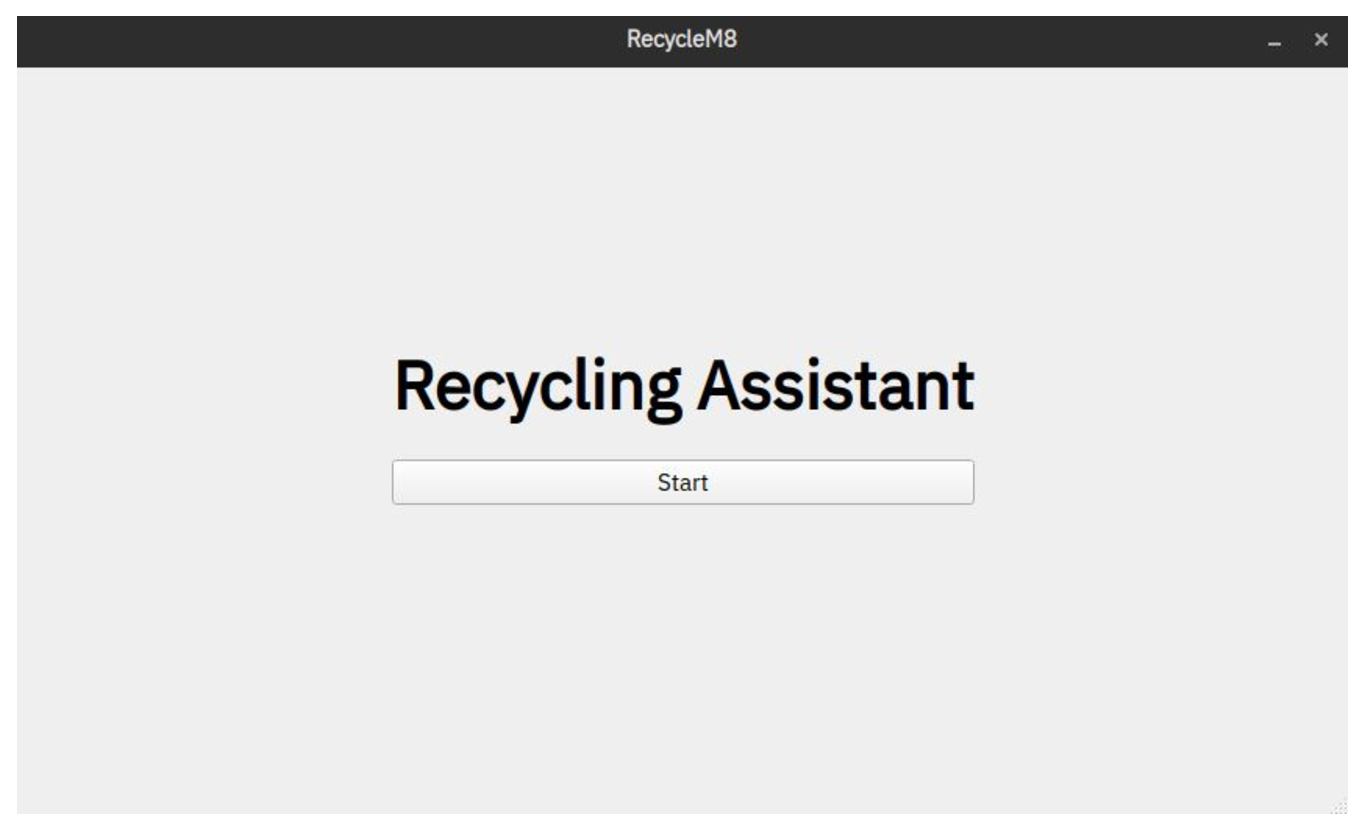
\includegraphics[width=0.48\textwidth]{images/start.eps}
    \caption{Initial Starting Page}
\end{figure}~\\

Once the "Start" button is clicked, they will be brought to the next menu. However, if the config file is valid (ie. does not fail the checks outlined in specification C: Reading the Configuration File), and the "skip\_start" settings flag is enabled, the application will skip directly to the scanning window, skipping the appearance of specification A: Initial Page.~\\

\subsection{Config File}
Upon application start, the settings/config file will be read. The settings/config file will read for and expect the following JSON values:~\\

\begin{itemize}
\item default\_source\_index: int
\item default\_source\_index: string
\item default\_source\_type: int
\item skip\_start: bool
\item model\_source: string
\item db\_usage: bool
\item db\_conn\_string: string
\item db\_user: string
\item db\_pw: string
\end{itemize}~\\

This will then be saved in memory in the form of an unordered\_map, for internal reference within the application.~\\

\subsection{Reading the Configuration File}
The settings/config file will be stored in the directory under the name "settings.json", in the JSON format. The conditions that would cause an error are the following:~\\

\begin{quote}
\subsubsection{File Not Found}~\\
If the configuration file is not in the directory, or if it has not been generated yet (ie. user's first launch).
\end{quote}

\begin{quote}
\subsubsection{JSON Initial Document Parse Failure}~\\
If the JSON parser encounters an issue while reading the file due to it being in an invalid JSON format, or corrupted.
\end{quote}

\begin{quote}
\subsubsection{JSON Validity Failure}~\\
If the JSON file is empty (typically resulting from unexpected closing/crashing while writing to the file).
\end{quote}

\begin{quote}
\subsubsection{JSON Objects Failure}~\\
If the JSON does not contain the required objects, or has an unexpectedly incorrect type.
\end{quote}

\begin{quote}
\subsubsection{JSON Value Failure}~\\
If the JSON does not contain valid values in its objects. The validation process of the JSON Values will be explained in a later specification.
\end{quote}~\\

In the case of an error, the user will be directed to the Settings Not Found menu, in specification C: Settings Not Found.~\\

\subsection{Settings Not Found}
If the application does not detect the settings/config file, or if it is either corrupted or unreadable (more details in specification C: Reading the Configuration File), the user will be notified that the application will launch with default parameters, while also being notified that it will generate a new Config file. This means that any existing file will be overwritten and regenerated with default values.~\\

If the user accepts (OK button), the application will proceed with the creation of a new Config file, while the user may also reject (Cancel button) to return to the previous screen, so that they may either try to manually adjust the JSON file, or save the parameter values before the file is overwritten.

\begin{figure}[h]
    \centering
    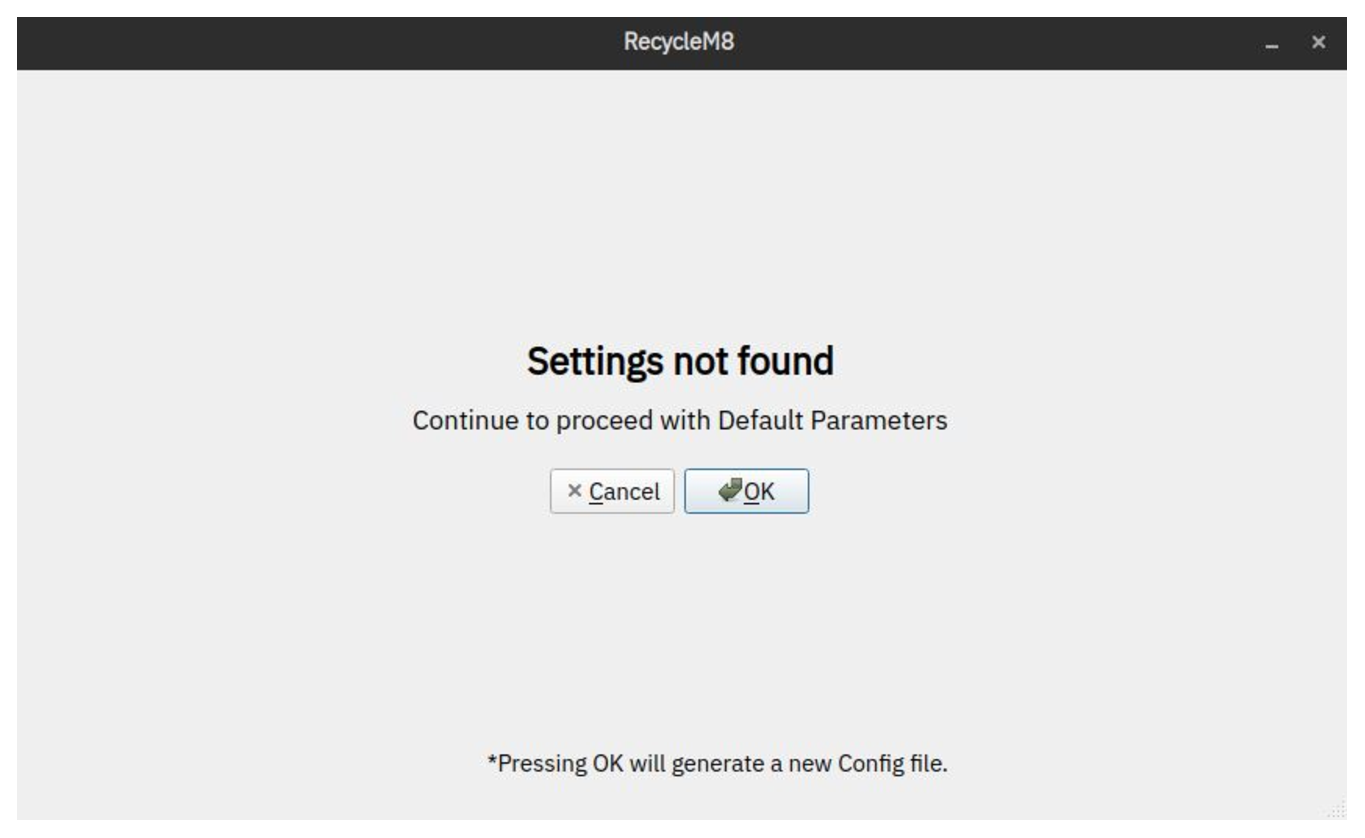
\includegraphics[width=0.48\textwidth]{images/settings_alert.eps}
    \caption{Settings Not Found}
\end{figure}~\\

\newpage
\subsection{Failure to Connect}
In the event that the application was not able to connect to the camera (usually occurring if the camera is not connected or offline), the user will be notified with a message box stating that there was an issue connecting to the camera.

They will see an empty detection screen, but will be able to access the settings menu in the top left corner (status bar). This will allow the user to adjust their set source.~\\

\begin{figure}[h]
    \centering
    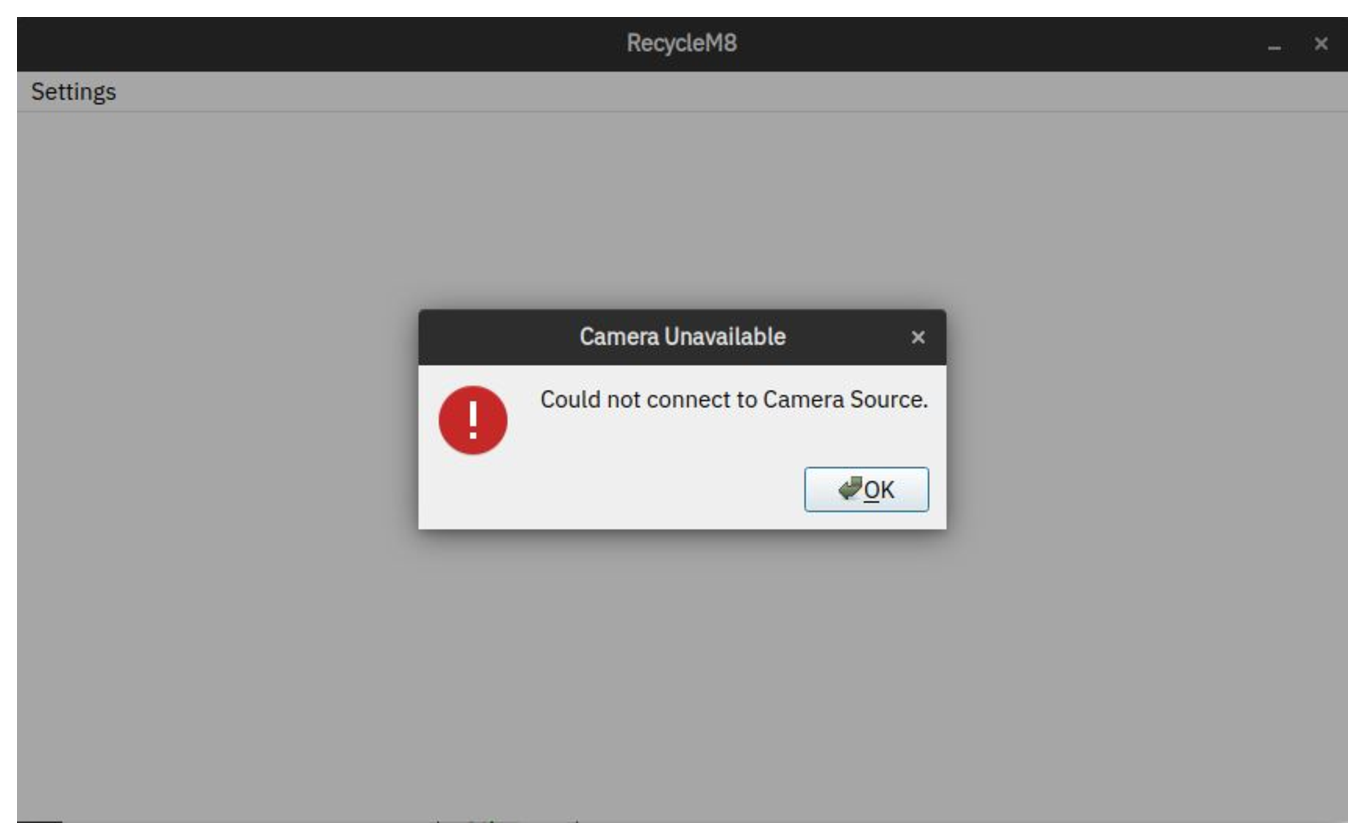
\includegraphics[width=0.48\textwidth]{images/camera_source_error.eps}
    \caption{Dialog Window Notification}
\end{figure}~\\
\begin{figure}[h]
    \centering
    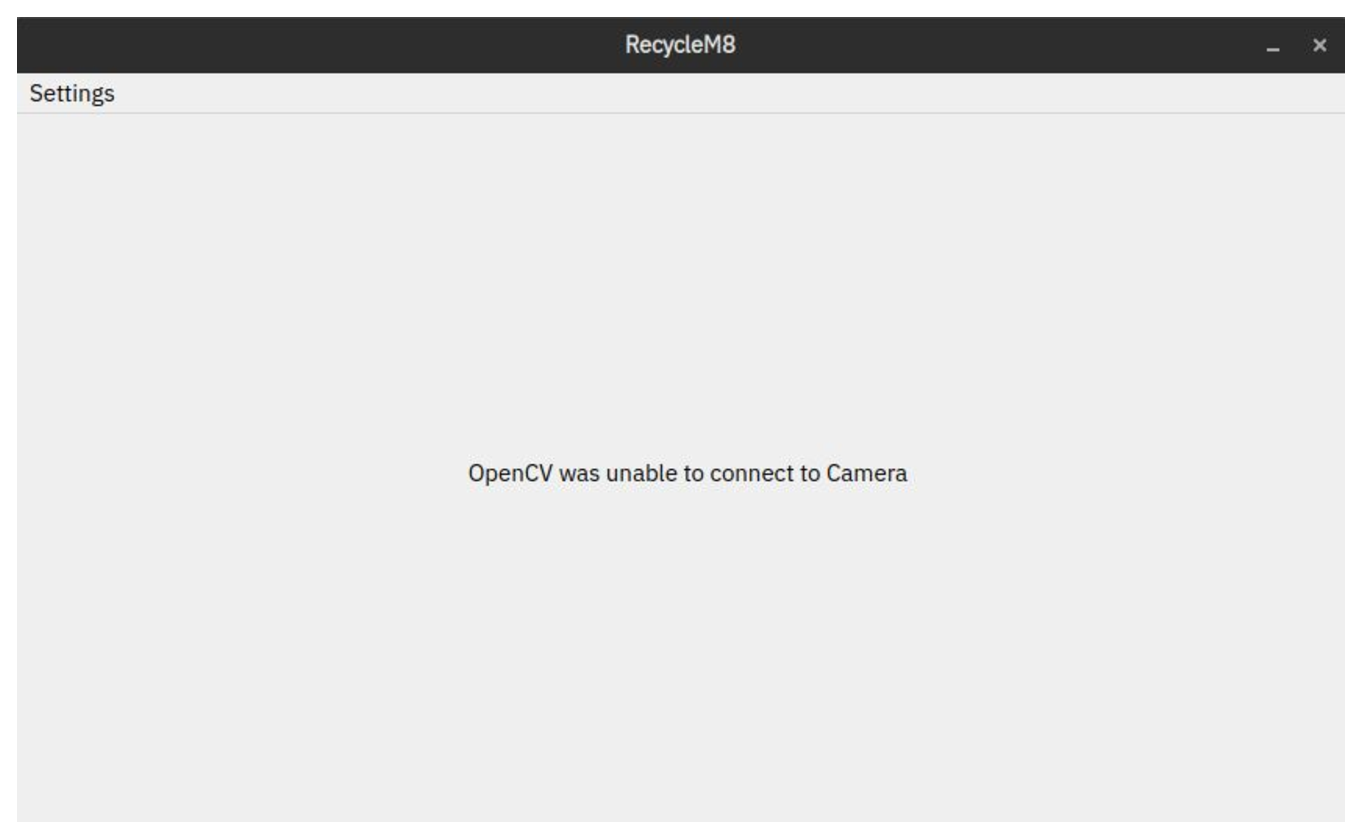
\includegraphics[width=0.48\textwidth]{images/camera_source_error_2.eps}
    \caption{After Dismissing Dialog Window Notification}

\end{figure}~\\

\newpage
\subsection{Detection/Scanner Screen}
The detection/scanner element takes up the vast majority of the application window estate. In this, a live camera feed is shown, based on the value assigned to the camera. ~\\

The default value is camera index 0 (the device index - 0 refers to the default camera for the system), however it can be assigned to another index, or to a video (ie. mp4 or webcam stream) through the settings menu.~\\

The image format should be correctly converted (from OpenCV's BGR output to RGB) for display in the application, and the webcam stream should not prevent or block the user from using any other user interface elements. In addition, the output frames will be appropriately resized to the window size in a 16:9 ratio.

\begin{figure}[h]
    \centering
    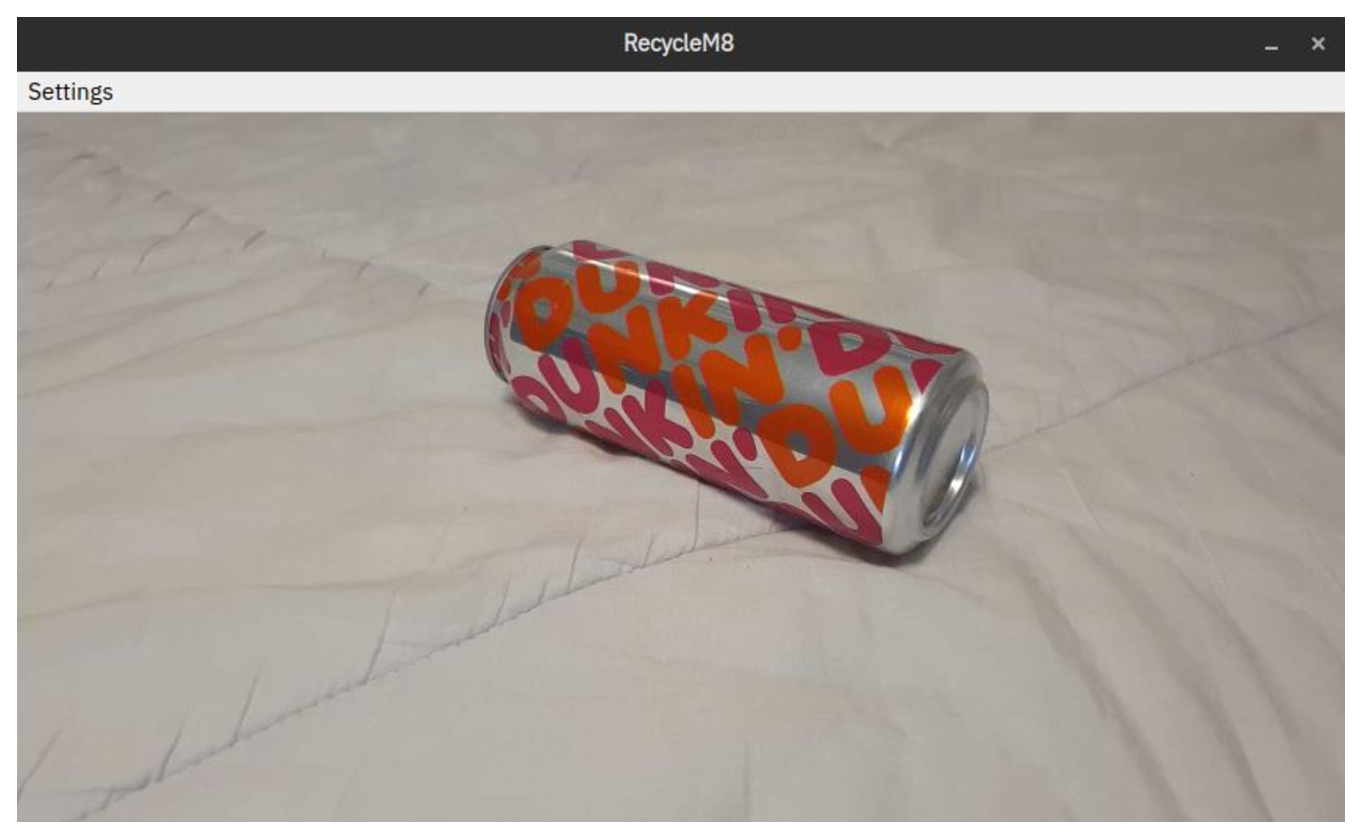
\includegraphics[width=0.48\textwidth]{images/scanner.eps}
    \caption{Scanner Main Screen}
\end{figure}~\\

\subsection{Object Detection}
When an object is detected by the model, a bounding box will be drawn on the object, alongside what it recognized, and the confidence level. In addition, the recycling category will be displayed. Unknown objects or the background should not be detected.~\\

\begin{figure}[h]
    \centering
    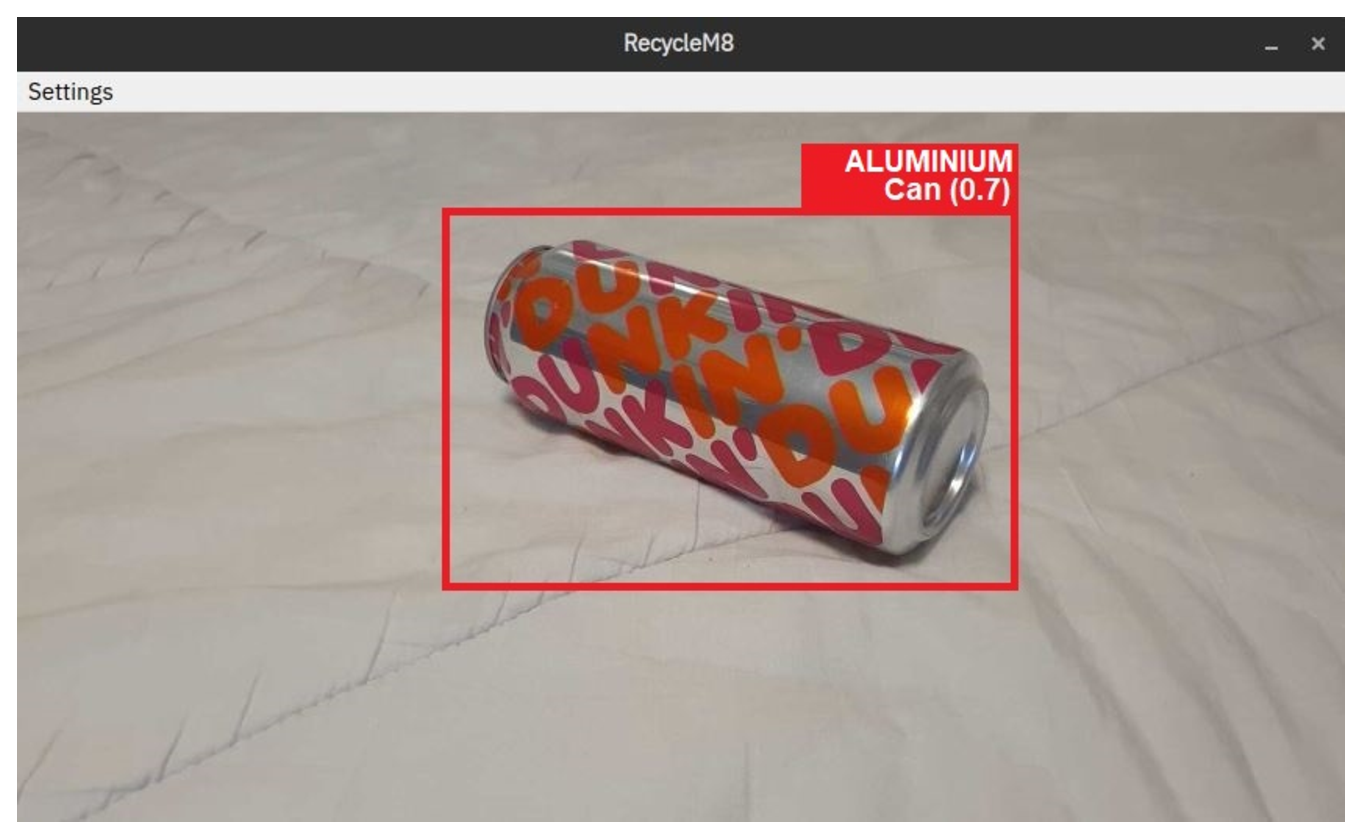
\includegraphics[width=0.48\textwidth]{images/object_detected.eps}
    \caption{-Placeholder- Successful Detection Frame}
\end{figure}~\\

\subsection{Settings Menu}
When the user clicks on "Adjust Settings" in the Settings Context Menu Button, they will be presented with a Settings Menu Window. In the window, they will see three tabs - one for OpenCV Settings, one for Application Settings, and one for Database Settings.~\\

\begin{figure}[h]
    \centering
    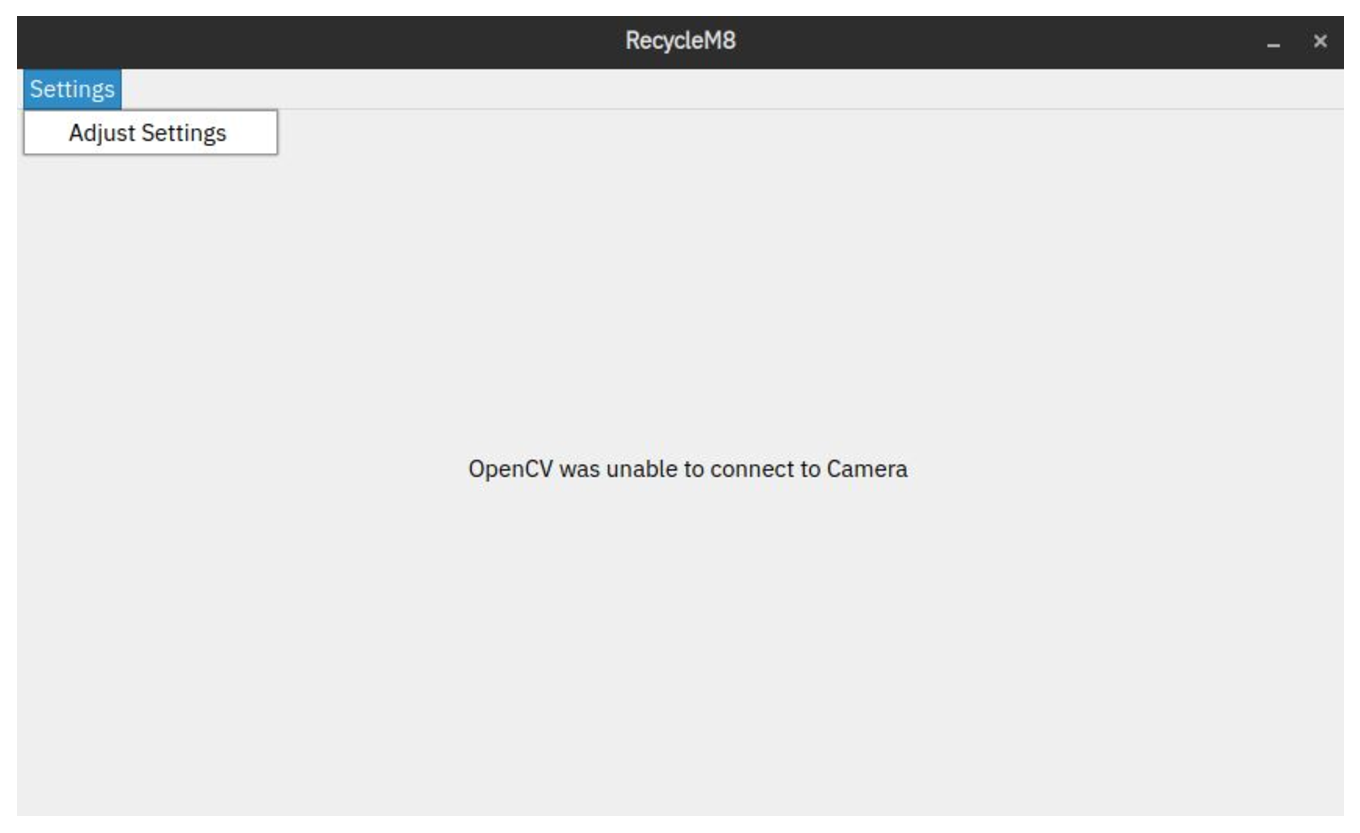
\includegraphics[width=0.48\textwidth]{images/settings_context_menu.eps}
    \caption{Settings Context Menu Option}
\end{figure}~\\

\subsection{OpenCV Settings}
This tab will contain settings related to OpenCV. The user will be able to choose between whether they would like to set their camera/stream based on the device index, or an IP address in the case of a webcam. The radio buttons will force the user to select one, and not both.~\\

\begin{figure}[h]
    \centering
    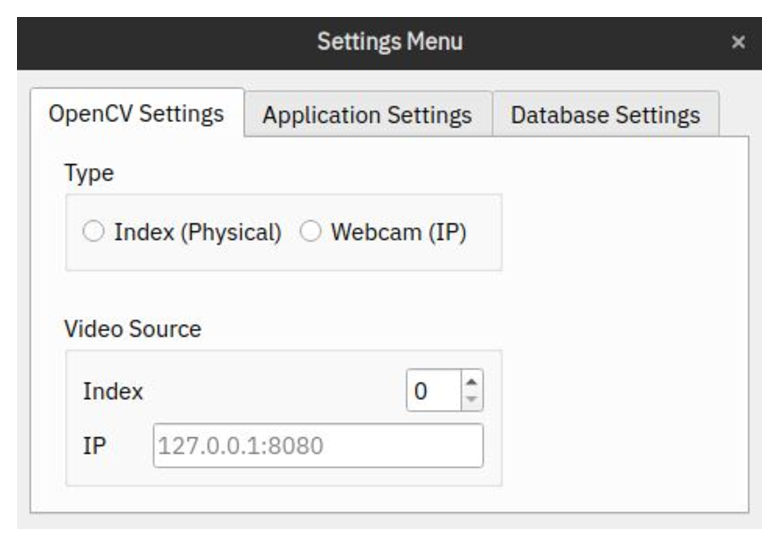
\includegraphics[width=0.48\textwidth]{images/settings_1.eps}
    \caption{OpenCV Settings Tab}
\end{figure}~\\

\subsection{Application Specific Settings}
This tab will contain settings related to the application. The user will be given the option to "Skip Start Sequence", which would make application starts skip directly to the detection screen.

In addition, advanced users may also specify if they would like to use a custom model source file.~\\

\begin{figure}[h]
    \centering
    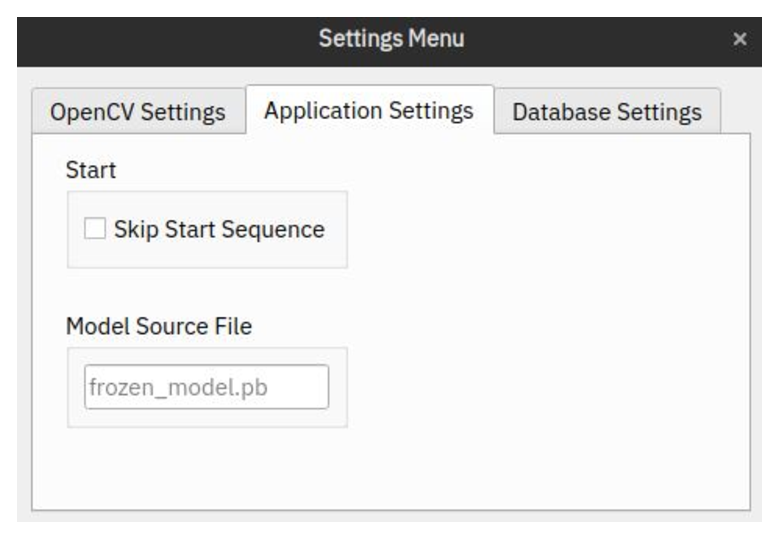
\includegraphics[width=0.48\textwidth]{images/settings_2.eps}
    \caption{Application Settings Tab}
\end{figure}~\\

\subsection{Database Settings}
This tab will contain settings related to the database. In this, the user may simply decide to choose to disable, or enable, the usage of database with regards to scans. The user may choose to do this if they would prefer not to have a database instance running, have no need for a database, or for privacy reasons.

While advanced users have the option to edit database related settings directly in the JSON, this will not be provided in the settings menu.~\\

\begin{figure}[h]
    \centering
    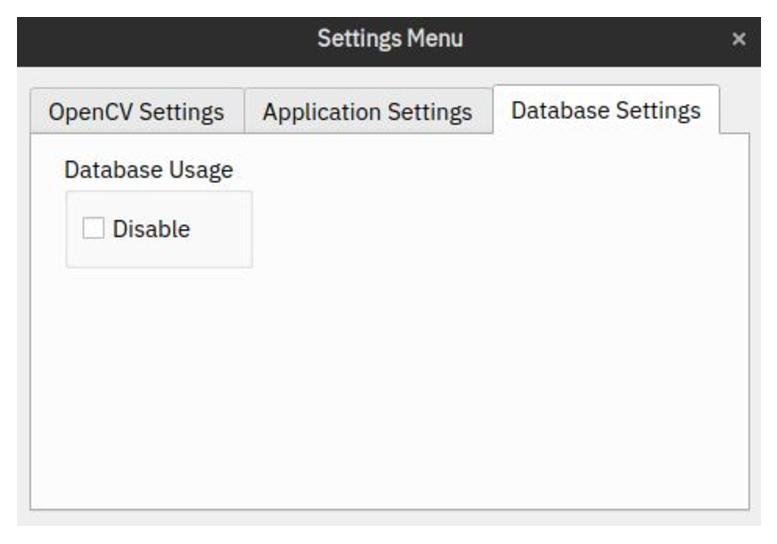
\includegraphics[width=0.48\textwidth]{images/settings_3.eps}
    \caption{Database Settings Tab}
\end{figure}~\\

\subsection{Statistics}
When the user clicks on "View Statistics" in the Statistics Context Menu Button, they will be presented with a Statistics Window. The window should be non-modal - as in, the user should still be able to interact with the other window at the same time while viewing statistics. In the window, they will see two tabs - one for session stats, and one for overall stats.~\\

\begin{figure}[h]
    \centering
    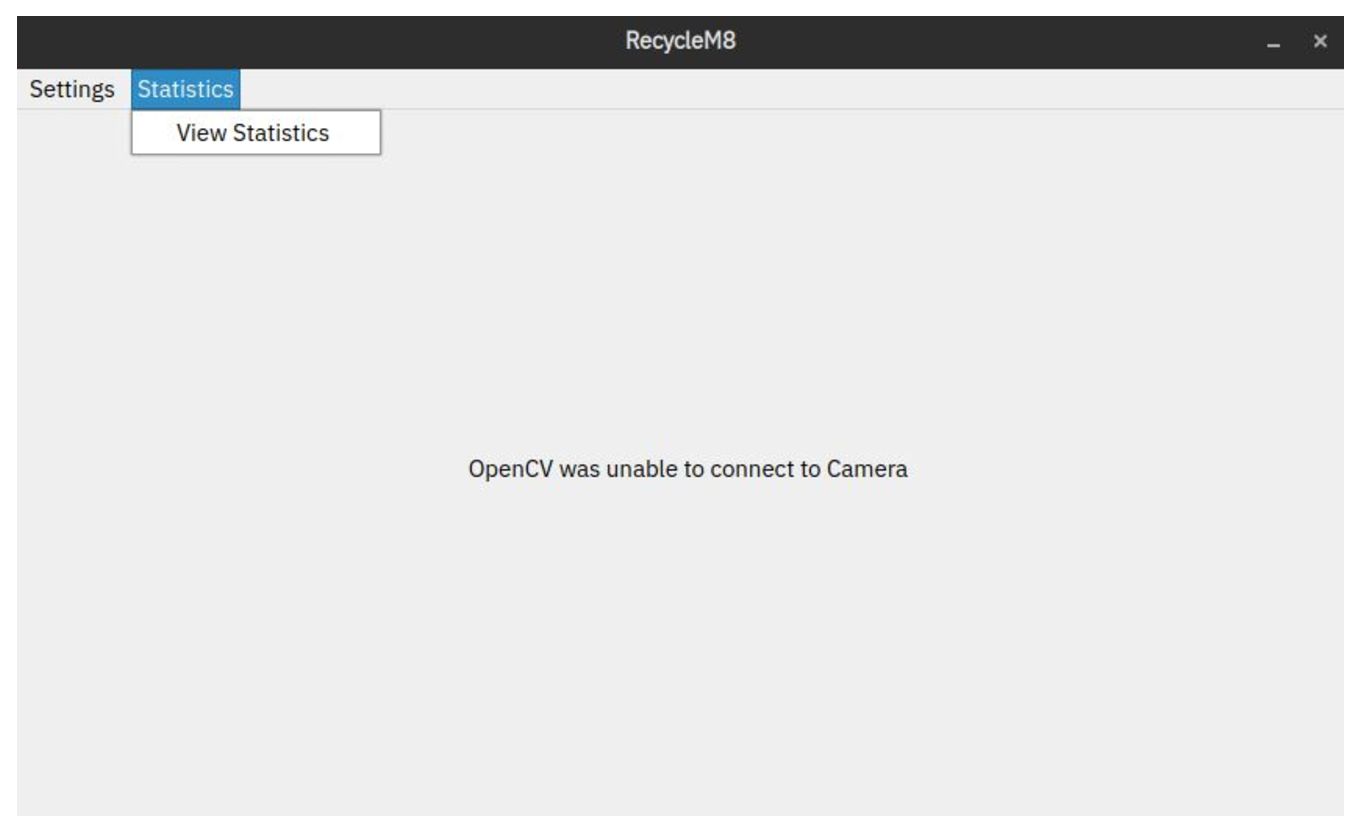
\includegraphics[width=0.48\textwidth]{images/stats_context_menu.eps}
    \caption{Statistics Context Menu}
\end{figure}~\\

\subsection{Session Statistics}
In the session stats window, they will see an "Overall Scan Count", and a "Categorical Scan Count". Overall scan count is self-explanatory - it is the number of times any object was scanned. Categorical scan count is the number of times an object from a category was scanned, divided by the overall scan count. The resulting percentage number is then rounded, and then fed into the progress bar.~\\

\begin{figure}[h]
    \centering
    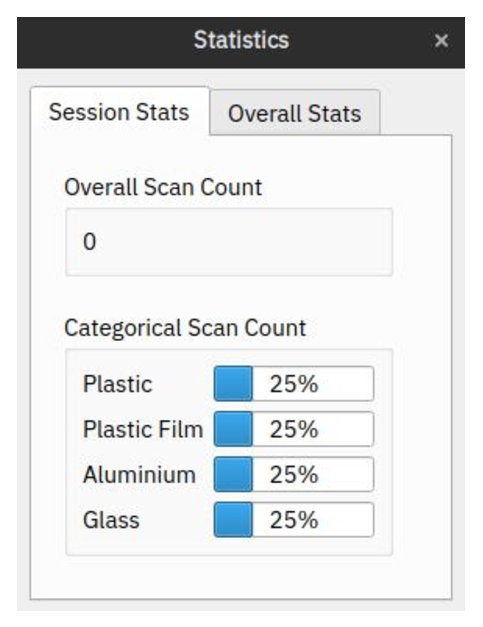
\includegraphics[width=0.48\textwidth]{images/statistics_session.eps}
    \caption{Database Settings Tab}
\end{figure}~\\

\subsection{Overall Statistics}
Similarly to the Session Statistics, the user will see an "Overall Scan Count", and a "Categorical Scan Count". However, this section is only functional if database is enabled, as it requires database data in order to operate.~\\

\begin{figure}[h]
    \centering
    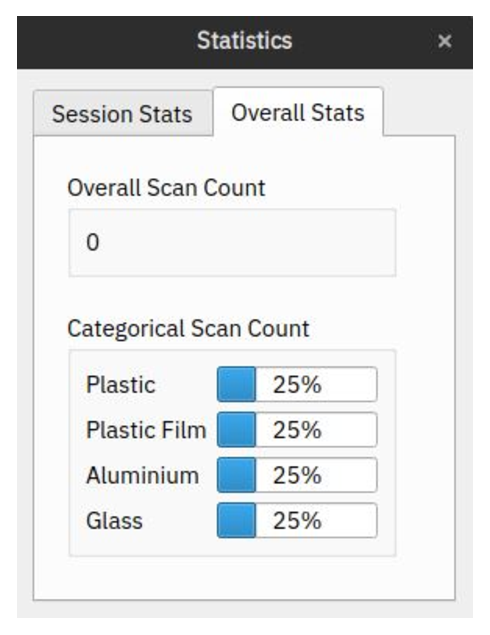
\includegraphics[width=0.48\textwidth]{images/statistics_overall.eps}
    \caption{Database Settings Tab}
\end{figure}~\\

\end{document}
